% Compile with pdfLaTeX (also compatible with standard TeX Live / Overleaf).
% Author: Ji Chengyu, G2608005K.
% Required evidence: screenshots/01-deployment.png, 02-wallet.png,
% 03-history.png, 04-invalid-input.png, 06-redemption.png,
% 07-backend.png, 08-render.png. Missing images are skipped with a warning.
% Keep the final compiled report within the assignment's 5-8 page range.
\documentclass[10pt,a4paper]{article}
\usepackage[T1]{fontenc}
\usepackage[utf8]{inputenc}
\usepackage{mathptmx}
\usepackage[margin=2cm]{geometry}
\usepackage{microtype}
\usepackage{graphicx}
\usepackage{tabularx,booktabs,array}
\usepackage{xcolor}
\usepackage{tikz}
\usetikzlibrary{positioning,arrows.meta}
\usepackage{placeins}
\usepackage{titlesec}
\usepackage[font=small,labelfont=bf]{caption}
\usepackage{hyperref}
\hypersetup{colorlinks=true,linkcolor=black,citecolor=black,urlcolor=blue!55!black,
  pdfauthor={Ji Chengyu},pdftitle={MicroInvest A Micro Investment Platform}}
\urlstyle{same}
\setlength{\parindent}{0pt}
\setlength{\parskip}{4pt}
\renewcommand{\baselinestretch}{1.0}
\renewcommand{\arraystretch}{1.10}
\titlespacing*{\section}{0pt}{10pt plus 2pt minus 1pt}{5pt}
\titlespacing*{\subsection}{0pt}{8pt plus 2pt minus 1pt}{4pt}
\setlength{\tabcolsep}{5pt}
\setcounter{topnumber}{3}
\setcounter{bottomnumber}{2}
\renewcommand{\topfraction}{0.90}
\renewcommand{\bottomfraction}{0.85}
\renewcommand{\textfraction}{0.08}
\graphicspath{{screenshots/}{report/screenshots/}}

\newcommand{\insertreportimage}[4]{%
  \begin{figure}[!htbp]
    \centering
    \includegraphics[width=#1,height=0.45\textheight,keepaspectratio]{#2}
    \caption{#3}\label{#4}
  \end{figure}%
}
\newcommand{\reportimage}[4][0.96\linewidth]{%
  \IfFileExists{screenshots/#2}{\insertreportimage{#1}{screenshots/#2}{#3}{#4}}{%
    \IfFileExists{report/screenshots/#2}{\insertreportimage{#1}{report/screenshots/#2}{#3}{#4}}{%
      \PackageWarning{MicroInvest}{Screenshot #2 not supplied yet}%
    }%
  }%
}

\title{MicroInvest\\\large A Micro Investment Platform}
\author{Ji Chengyu\\Student ID G2608005K\\\small SC6113 Individual Assignment Financial Decentralized Application}
\date{7 October 2026}
\begin{document}
\begin{center}
{\Large\bfseries MicroInvest\par}
{\large A Micro Investment Platform\par}
\vspace{4pt}
Ji Chengyu \quad Student ID G2608005K\\
SC6113 Individual Assignment Financial Decentralized Application\\
7 October 2026
\end{center}

\section{Introduction}

MicroInvest is an educational financial DApp for investing beginners. Users deposit Sepolia test ETH into one pool, receive internal shares, inspect their position and redeem principal at any time. A Solidity contract connects to an English interface and Flask backend, deployed at \href{https://sc6113-developemnt-coursework.onrender.com/}{MicroInvest on Render}.

One ETH equals one share, including fractions. Funds remain in the contract for withdrawals, with no market investment, yield, platform fee or administrator. Users pay network gas separately. The prototype demonstrates ownership, accounting and confirmation without suggesting investment returns.

\section{Problem Statement}

A beginner must distinguish contributions, ownership and transaction cost, as well as wallet approval from blockchain confirmation. Unclear balances or withdrawal conditions make it difficult to understand where funds are held and how to recover them.

MicroInvest addresses this through fractional deposits, visible share conversion and partial or full redemption. On-chain state determines each account's entitlement; confirmed events provide history. Market allocation, diversification and capital growth are outside the prototype's scope.

\section{Objectives}

The objectives are to implement exact fractional ownership in Solidity; enable MetaMask connection and account selection; support deposits and caller-bound principal redemption; provide useful Flask queries for positions, events and receipts; and distinguish validation errors, wallet rejection, pending transactions and mined results. Evaluation covers contract authorization, accounting, common failure paths, interface behavior and measured gas. The source, deployment details, README and report follow the assignment requirements \cite{assignment}.

\section{System Architecture}

The application separates reads from signed writes. The browser obtains public configuration, pool state, individual positions and transaction history from Flask. Web3.py queries the configured Sepolia JSON-RPC service. Deposits and redemptions are constructed with ethers and submitted through MetaMask after user approval. The backend does not sign transactions or hold the user's private key.


\begin{figure}[htbp]
\centering
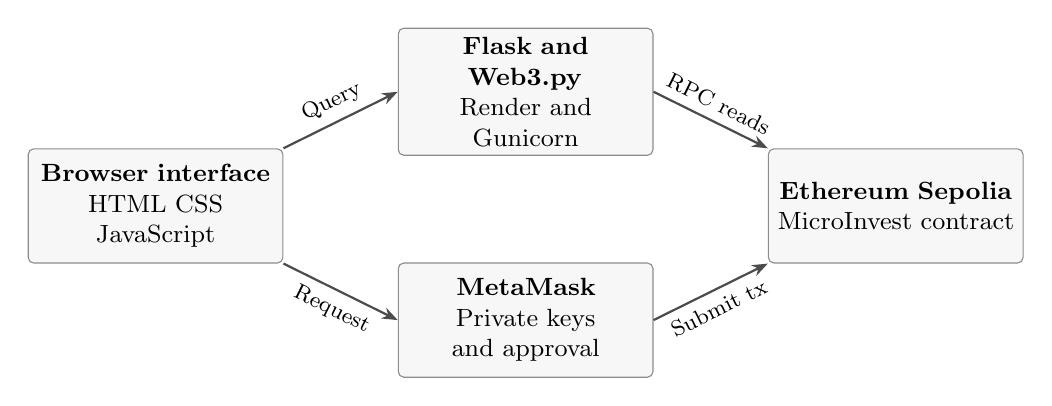
\begin{tikzpicture}[
  block/.style={draw=black!45,fill=black!3,rounded corners=2pt,
    text width=3.0cm,minimum height=1.45cm,align=center,font=\small},
  link/.style={-{Stealth[length=2mm]},draw=black!70,thick},
  note/.style={font=\footnotesize,align=center}]
\node[block] (browser) at (0,0) {\textbf{Browser interface}\\HTML CSS JavaScript};
\node[block] (backend) at (4.7,1.45) {\textbf{Flask and Web3.py}\\Render and Gunicorn};
\node[block] (wallet) at (4.7,-1.45) {\textbf{MetaMask}\\Private keys and approval};
\node[block] (chain) at (9.4,0) {\textbf{Ethereum Sepolia}\\MicroInvest contract};
\draw[link] (browser.north east) -- node[note,above,sloped] {Query} (backend.west);
\draw[link] (backend.east) -- node[note,above,sloped] {RPC reads} (chain.north west);
\draw[link] (browser.south east) -- node[note,below,sloped] {Request} (wallet.west);
\draw[link] (wallet.east) -- node[note,below,sloped] {Submit tx} (chain.south west);
\end{tikzpicture}
\caption{System architecture and the boundary between queries and wallet signing.}
\label{fig:architecture}
\end{figure}

The contract is the source of truth. No database is used; Flask reconstructs confirmed balances and events from the chain after restart. Browser storage retains transaction hashes and preferred accounts per pool/network but cannot grant permissions or establish balances.

Every blockchain API query verifies the configured chain and exact deployed runtime bytecode. Pool and position calls use a snapshot block. History scans are bounded to 5,000 blocks per request, with log requests split into chunks of at most 1,000 blocks. An exclusive block/log-index cursor supports older pages without repeating events when several records share a block.

\section{Technologies Used}

\begin{table}[htbp]\centering\small
\caption{Technologies and their roles}\label{tab:technology}
\begin{tabularx}{\linewidth}{@{}>{\raggedright\arraybackslash}p{0.19\linewidth}>{\raggedright\arraybackslash}p{0.3\linewidth}>{\raggedright\arraybackslash}X@{}}
\toprule
\textbf{Layer} & \textbf{Technology} & \textbf{Role} \\
\midrule
Contract & Solidity 0.8.30 & Custody, shares, caller authorization and events \\
Development tools & Node.js 24, Hardhat 3, pnpm & Compilation, local chain, contract and browser tests \\
Browser & HTML, CSS, JavaScript, ethers 6 & Responsive pages and wallet transaction construction \\
Backend & Python 3.12, Flask, Web3.py & Validated read-only blockchain APIs \\
Wallet and network & MetaMask, Ethereum Sepolia & User approval, signing and testnet execution \\
Hosting and workflow & Render, Gunicorn, GitHub, VS Code & Web hosting, source control and development \\
\bottomrule
\end{tabularx}
\end{table}

Node.js supports development and testing; the deployed service runs Python and Gunicorn. Committed artifacts and the ethers bundle avoid Solidity compilation or Node.js installation during the web build. Gunicorn supplies the production WSGI server \cite{flask,render}.

\section{Smart Contract Design}

\texttt{MicroInvest.sol} stores \texttt{shares[address]} and \texttt{totalShares} as unsigned integer units. One displayed share has 18 decimal places, so a deposit's wei value directly equals the credited share units. This avoids rounding in conversion. The supported accounting invariants are that total shares equal the sum of user shares, each user's redeemable wei equals their shares, and contract balance is at least the recorded principal.

\begin{table}[htbp]\centering\small
\caption{Contract methods and validation}\label{tab:contract}
\begin{tabularx}{\linewidth}{@{}>{\raggedright\arraybackslash}p{0.3\linewidth}>{\raggedright\arraybackslash}p{0.37\linewidth}>{\raggedright\arraybackslash}X@{}}
\toprule
\textbf{Method} & \textbf{State transition} & \textbf{Validation} \\
\midrule
\texttt{deposit()} & Credit the caller and total shares by \texttt{msg.value} & Deposit is greater than zero \\
\texttt{withdraw(amountWei)} & Debit caller and total; send the same amount to caller & Positive amount and sufficient caller shares \\
\texttt{withdrawAll()} & Redeem the caller's entire nonzero position & Caller has shares \\
\texttt{shares(address)} and \texttt{totalShares()} & Read ledger balances & No state change \\
\bottomrule
\end{tabularx}
\end{table}

For example, depositing 0.003 ETH credits 0.003 shares. Redeeming 0.001 debits exactly that amount, leaving 0.002. Full redemption then clears the position. Gas is charged to the wallet separately, so redeeming all principal does not restore gas previously spent.

Authorization follows \texttt{msg.sender}: a transaction changes only the calling account's entitlement. Shares cannot be transferred. The deploying account receives no withdrawal privilege, and the contract has no owner, pause or upgrade function. These decisions keep the participant's rules explicit, while also removing administrative recovery options.

Withdrawals check entitlement, debit state and then transfer ETH. A reentrancy lock blocks nested entry; a failed transfer reverts the entire operation, including the ledger debit. This follows the checks-effects-interactions principle described in Solidity's security guidance \cite{solidity}. Tests use both a receiver that refuses ETH and a receiver that attempts a nested withdrawal.

\texttt{Deposited} and \texttt{Withdrawn} events contain an indexed investor, the wei amount and resulting shares. Successful events support confirmed history. A wallet rejection or reverted operation creates no successful business event. ETH forcibly received outside \texttt{deposit()} is reported as excess balance and creates no new shares or yield.

The compiler optimizer is enabled with 200 runs. Contract operations change a fixed amount of storage and do not loop over investors. Gas measurements are reported in Section 9; they are evidence from specific transactions rather than a guarantee of future cost.

\section{Application Design}

The dark English overview explains the testnet, fixed share conversion, zero platform fee and separate gas cost. It combines deposit/redemption controls with personal shares, redeemable principal and wallet balance. Separate controls support partial redemption and full exit. Labels, visible feedback and responsive layouts support the intended beginner audience.

A connected wallet address opens an account menu on both the overview and activity page. The list uses addresses actually exposed by \texttt{eth\_accounts}. Manage accounts requests wallet permission after a user click; selecting an account refreshes its position and history. Before signing, the application confirms that the selected account is still authorized and uses \texttt{getSigner(selectedAddress)}, even when it is not the first address returned. Provider account/network events and permission requests follow the interfaces in \cite{provider,permissions}.

The overview shows the five newest confirmed records. View all activity opens a separate page that initially shows 20 records and loads older cursor pages. Links point to actual Sepolia transactions. The complete history page also accepts a public wallet address for read-only viewing.


\begin{figure}[htbp]
\centering
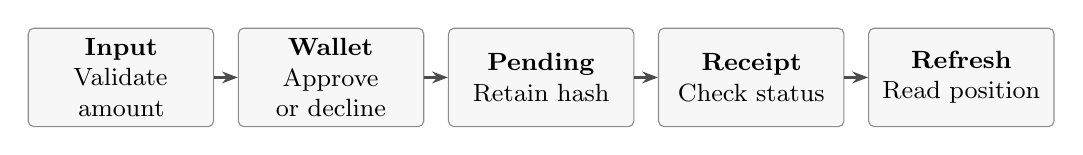
\begin{tikzpicture}[
  stage/.style={draw=black!45,fill=black!3,rounded corners=2pt,
    text width=2.12cm,minimum height=1.25cm,align=center,font=\small},
  link/.style={-{Stealth[length=2mm]},draw=black!70,thick}]
\node[stage] (input) {\textbf{Input}\\Validate amount};
\node[stage,right=3mm of input] (wallet) {\textbf{Wallet}\\Approve or decline};
\node[stage,right=3mm of wallet] (pending) {\textbf{Pending}\\Retain hash};
\node[stage,right=3mm of pending] (receipt) {\textbf{Receipt}\\Check status};
\node[stage,right=3mm of receipt] (refresh) {\textbf{Refresh}\\Read position};
\draw[link] (input) -- (wallet);
\draw[link] (wallet) -- (pending);
\draw[link] (pending) -- (receipt);
\draw[link] (receipt) -- (refresh);
\end{tikzpicture}
\caption{Transaction feedback distinguishes wallet approval from a mined result.}
\label{fig:lifecycle}
\end{figure}

A rejected wallet request is shown as declined. A submitted hash is pending until a receipt is available. A successful receipt refreshes the position; a failed receipt reports a revert. If confirmation is delayed, the hash is retained for later checking. Account changes clear previous data, and older asynchronous responses cannot overwrite the new account's position.

\reportimage{02-wallet.png}{Connected MetaMask account on Sepolia with a second authorized account available in the account menu.}{fig:02-wallet}

\section{Implementation}

The repository contains the business contract and adversarial tests, an exported ABI/bytecode artifact, Flask routes, the blockchain query service, HTML templates and JavaScript modules. The browser actively calls \path{/api/config}, \path{/api/pool}, \path{/api/position/<wallet>}, \path{/api/history/<wallet>} and \path{/api/transactions/<hash>}. Flask validates addresses, hashes and pagination parameters and returns amounts as decimal strings. JavaScript uses \texttt{BigInt} for wei rather than floating-point arithmetic.

The MetaMask deployment page lets the user deploy without supplying a private key to Flask. Public deployment metadata records the address and deployment block. On Render, the build installs \texttt{requirements.txt} and Gunicorn starts \texttt{app:app}. Environment configuration identifies Sepolia, its RPC endpoint and this deployed pool; \texttt{/healthz} checks process readiness, while \texttt{/api/pool} verifies real blockchain access.

\FloatBarrier
\section{Testing and Results}

Automated testing combines contract tests, backend unit tests, exact-amount tests and an actual browser against Flask and a local Hardhat chain. The browser's EIP-1193 wallet is simulated. Backend unit tests mock the RPC boundary; the integration suite supplies real local state changes. These results do not by themselves prove real MetaMask behavior or hosted operation.

\begin{table}[htbp]\centering\small
\caption{Automated testing results}\label{tab:tests}
\begin{tabularx}{\linewidth}{@{}>{\raggedright\arraybackslash}p{0.2\linewidth}>{\raggedright\arraybackslash}p{0.25\linewidth}>{\raggedright\arraybackslash}X@{}}
\toprule
\textbf{Suite} & \textbf{Result} & \textbf{Evaluation covered} \\
\midrule
Contract & 12 passed, 6 October & Exact units, isolation, transfer rollback, reentrancy and a 40-operation accounting sequence \\
Flask backend & 17 passed, 7 October & Validation, public configuration, bytecode/network checks, receipt states and cursor boundaries \\
Amount and error handling & 4 passed, 7 October & One wei, large integers, invalid decimals and safe wallet errors \\
Browser integration & 19 checks passed, 7 October & Deposit/exit flow, account selection/signing, five-record preview, pagination, mobile layout and RPC failure \\
\bottomrule
\end{tabularx}
\end{table}

For invalid input, zero, negative, exponential, nonnumeric and over-precision values are rejected. Excess redemption cannot spend another account's shares. Refusing a wallet request leaves contract state unchanged. Simulated network changes disable writes; an RPC outage displays an unavailable position instead of inventing a zero balance. At a 390-pixel viewport, the document and account menu remain within the screen width.

I completed functional testing on Render with MetaMask. Independent read-only checks on 7 October returned HTTP 200 for the home, configuration, health and pool endpoints, identifying chain 11155111 and the expected contract. That snapshot showed a solvent pool with zero principal and eight confirmed participant events. A later history screenshot contains nine records, including a subsequent 0.04 ETH deposit. The supplied API snapshot shows 0.04 ETH principal and balance at block 11857366, with zero excess and \texttt{solvent: true}. The later confirmed redemption at block 11857372 shows zero personal shares and redeemable principal. These screenshots document different blocks rather than conflicting balances.

\begin{table}[htbp]\centering\small
\caption{Confirmed Sepolia principal lifecycle}\label{tab:live}
\begin{tabularx}{\linewidth}{@{}>{\raggedright\arraybackslash}p{0.39\linewidth}>{\raggedright\arraybackslash}p{0.18\linewidth}>{\raggedright\arraybackslash}p{0.17\linewidth}>{\raggedright\arraybackslash}X@{}}
\toprule
\textbf{Observed Sepolia operation} & \textbf{Amount in ETH} & \textbf{Shares after} & \textbf{Block} \\
\midrule
Deposit & 0.003 & 0.003 & 11856700 \\
Partial redemption & 0.001 & 0.002 & 11856703 \\
Full redemption & 0.002 & 0 & 11856705 \\
\bottomrule
\end{tabularx}
\end{table}

All three receipts report success. Their full transaction hashes and raw API evidence are retained in \path{docs/evidence/live-validation-2026-10-07.json}. The chain record proves the debit/credit sequence; screenshots illustrate the corresponding user experience.

\begin{table}[htbp]\centering\small
\caption{Gas used in separate local and Sepolia observations}\label{tab:gas}
\begin{tabularx}{\linewidth}{@{}>{\raggedright\arraybackslash}p{0.35\linewidth}>{\raggedright\arraybackslash}p{0.25\linewidth}>{\raggedright\arraybackslash}X@{}}
\toprule
\textbf{Operation} & \textbf{Local receipt gas} & \textbf{Observed Sepolia receipt gas} \\
\midrule
Deposit & 71,884 & 245,994 \\
Partial redemption & 50,282 & 53,700 \\
Full redemption & 50,272 & 50,912 \\
\bottomrule
\end{tabularx}
\end{table}

These are separate observations with different transaction amounts and execution environments. The local cases used 0.01 ETH for the first deposit, 333 wei for partial exit and 999 wei for full exit. Actual fee is receipt gas multiplied by effective gas price. The three Sepolia transactions cost 0.000622855710866760, 0.000132064592365200 and 0.000127495073925600 ETH respectively. No throughput benchmark or novice-user study was conducted.

\reportimage{03-history.png}{Complete activity page showing confirmed deposits and redemptions, including the 0.003 ETH deposit, 0.001 ETH partial redemption and 0.002 ETH full exit.}{fig:03-history}

\reportimage[0.46\linewidth]{07-backend.png}{Pool API at block 11857366: 0.04 ETH principal and contract balance, zero excess and solvent true, before the later redemption.}{fig:07-backend}

\reportimage{06-redemption.png}{Confirmed redemption at block 11857372 with zero personal shares and zero redeemable principal.}{fig:06-redemption}

\subsection*{Deployment and live evidence}

The pool is deployed at \texttt{0xE560121978f80c390f6B0d091E9579A2812Cb3DD} on Sepolia. Its creation receipt is successful in block 11856501 and used 1,814,581 gas. Exact runtime bytecode matches the committed artifact. The deploying account is an ordinary participant.

\href{https://sepolia.etherscan.io/tx/0x45dba804763f4d53c4da30957b3d4da0f02dd15eecb65762a904926f99efd2ea}{Deployment transaction} | \href{https://sepolia.etherscan.io/tx/0x0304792edcd32dc589e6e5c7756f86fdc33a283c295b78772a8e323b4d490798}{Deposit transaction} | \href{https://sepolia.etherscan.io/tx/0xcb3ebbe7044daf65d6129d01cb936cfaa9ccc8553b347ebccbe13a09b477804e}{Partial redemption} | \href{https://sepolia.etherscan.io/tx/0xe47ab65933833624b02fddd362fcce5ade0c734d1626790b3239831ff4f06e9a}{Full redemption}

\reportimage{01-deployment.png}{Deployment confirmation showing Sepolia chain ID 11155111, the deployed contract address and block 11856501.}{fig:01-deployment}

\reportimage{04-invalid-input.png}{A negative deposit amount of -1 ETH with a message requiring a positive ETH amount.}{fig:04-invalid-input}

\reportimage{08-render.png}{Render deployment succeeded and Live for commit b65f9c3, with Gunicorn startup logs and the public service URL.}{fig:08-render}

The interface validates exact amounts and wallet context; Solidity independently enforces positive values and caller ownership. Flask rejects malformed query parameters and exposes no write endpoint. Private keys stay in MetaMask; RPC credentials stay server-side. Sanitized errors and a Content Security Policy reduce exposure and unsafe content.

Addresses, events and amounts remain public despite the absence of a database. No identity profiles are collected. The interface explains test ETH and the absence of returns. Usability observations come from functional checks and my walkthrough; no controlled beginner study was conducted.

\FloatBarrier
\section{Challenges Encountered}

Integer wei and string responses solved cross-layer decimal precision. Separate signing, pending, mined and unknown states prevented premature success messages. Bounded history queries and block/log-index cursors handled RPC limits and same-block events. Account selection required the selected authorized signer; separating public artifacts from runtime secrets kept Render deployment reproducible.

\section{Limitations}

The prototype holds principal without a market strategy, diversification or yield. One mined confirmation is sufficient for its feedback but is not chain finality. Public RPC availability and wallet behavior affect operation, and old inactive history can require several page requests. There is no formal external security audit, load test or beginner usability study. With no administrator or upgrade mechanism, there is no administrative rescue path for excess ETH. The testnet prototype is not evaluated for custody of real savings.

\section{Future Improvements}

Future work includes beginner usability testing, clearer delayed-transaction recovery, an event index with reorganization handling and multiple wallet providers. Real investment strategies, transferable tokens or additional assets require a separate specification, risk model and security review.

\section{Conclusion}

MicroInvest implements the selected micro-investment workflow through exact fractional shares, wallet-authorized transactions and caller-bound principal exit. Flask provides real contract queries and event history, while MetaMask signs writes. Automated tests cover accounting and failure cases, and the deployed Sepolia/Render integration supports the demonstrated lifecycle. The result meets the financial DApp learning objectives within a clearly stated educational scope.

\FloatBarrier
\begin{thebibliography}{9}
\small
\setlength{\itemsep}{2pt}
\bibitem{assignment} SC6113 Individual Assignment Financial Decentralized Application.
Supplied coursework Word document, Sections III and VI--XI.
\bibitem{solidity} Solidity 0.8.30. \emph{Security Considerations}.
\url{https://docs.soliditylang.org/en/v0.8.30/security-considerations.html}.
\bibitem{provider} Ethereum Improvement Proposals. \emph{EIP-1193 Ethereum Provider JavaScript API}.
\url{https://eips.ethereum.org/EIPS/eip-1193}.
\bibitem{permissions} Ethereum Improvement Proposals. \emph{EIP-2255 Wallet Permissions System}.
\url{https://eips.ethereum.org/EIPS/eip-2255}.
\bibitem{flask} Flask 3.1 documentation. \emph{Deploying to Production}.
\url{https://flask.palletsprojects.com/en/stable/deploying/}.
\bibitem{render} Render documentation. \emph{Deploy a Flask App}.
\url{https://render.com/docs/deploy-flask}.
Online documentation accessed 7 October 2026.
\end{thebibliography}
\end{document}
